%!TEX root = ../../../super_main.tex

\section{Bug Splash Screen}
\label{sec:bug_splash_screen}

We have implemented a bug splash screen with the hope of displaying a more meaningful and assuring message in case of uncaught exceptions rather than just letting the application crash. The bug splash screen also prints a stack trace of the GUI thread in order to help future developers whom might have forgotten to attach a debugger the one time some rare race condition occurred. An example can be seen in \figref{fig:bug_splash_screen_example}.\\

The bug splash screen works by setting an \androidinline{UncaughtExceptionHandler} on the shared GUI thread of an application every time a \androidinline{GirafActivity} is created. An existing \androidinline{UncaughtExceptionHandler} would simply be overridden. A special bug splash \androidinline{Activity} will then be brought to the front in case the \androidinline{UncaughtExceptionHandler} catches an \androidinline{Exception}.

\begin{figure}[!htbp]
        \centering
        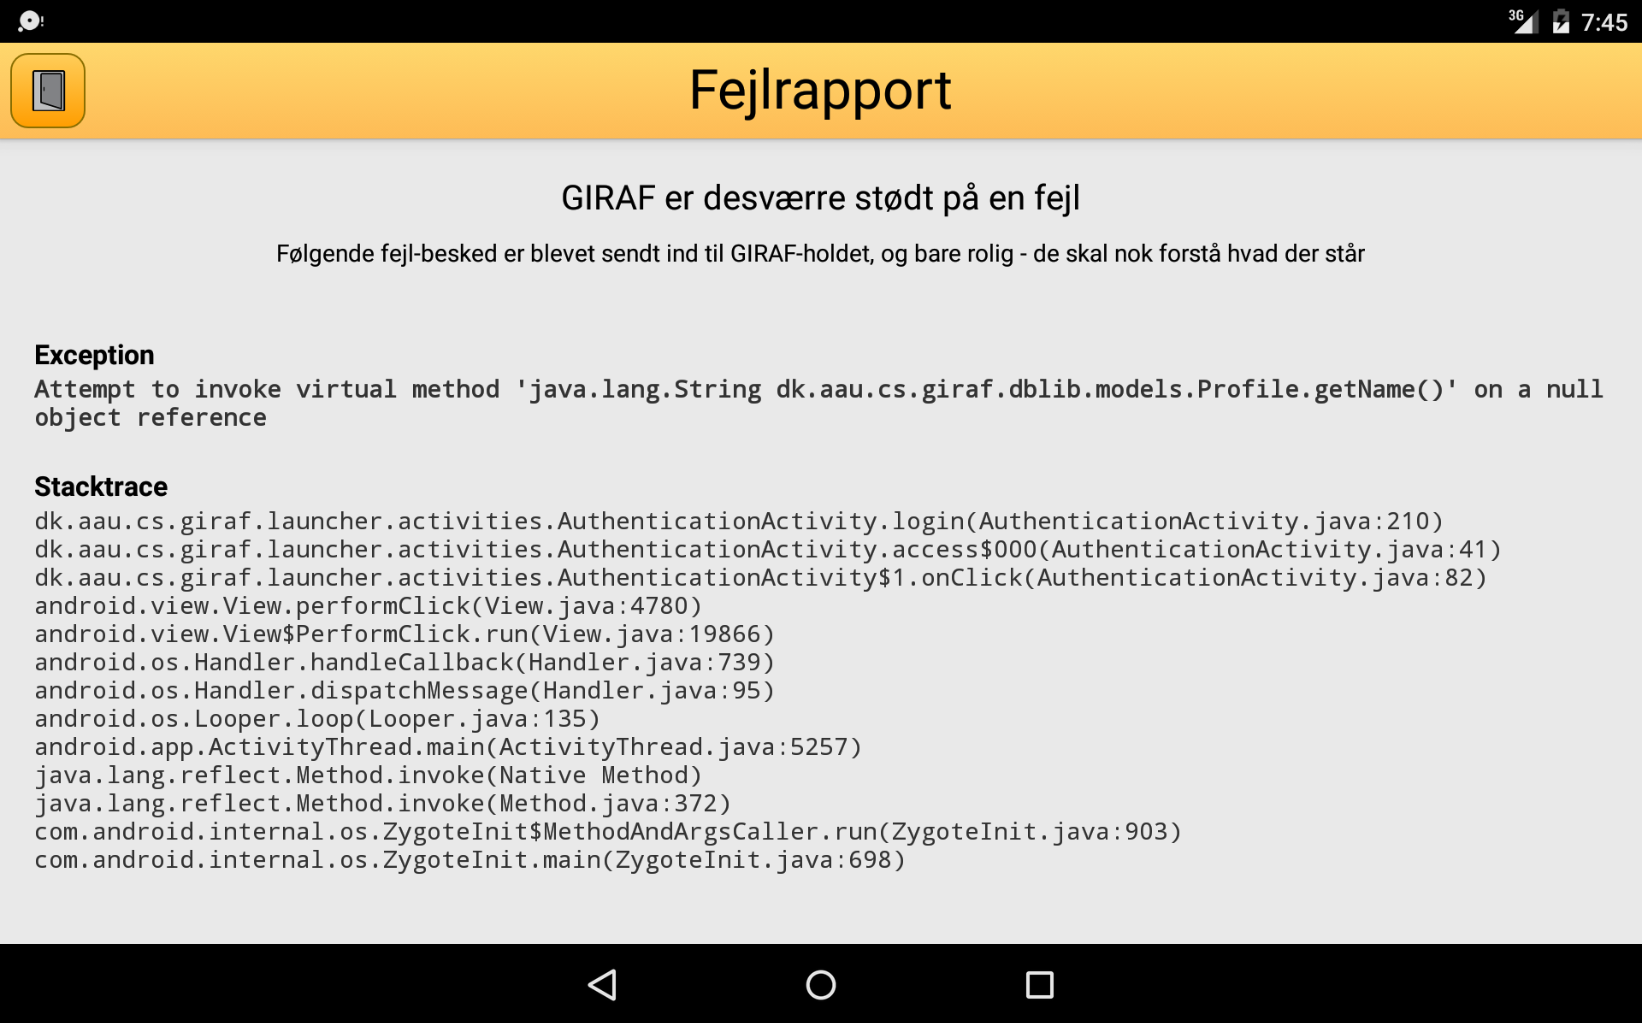
\includegraphics[width=1\textwidth]{sprint_four/bug_splash_screen}
        \caption{Bug splash screen example}
        \label{fig:bug_splash_screen_example}
\end{figure}

\subsection{Only GUI thread} 
The bug splash screen only works for the main thread of the application, e.i. the GUI thread, because it would be too cumbersome to apply an \androidinline{UncaughtExceptionHandler} to every new thread started. Some background threads, i.e. not the GUI thread, might be managed indirectly by the Android framework e.g. in the \androidinline{doInBackground} method of an \androidinline{AsyncTask}. We could in theory subclass \androidinline{AsyncTask} and provide an implementation of \androidinline{doInBackground} which would set an \androidinline{UncaughtExceptionHandler} on the background thread managed by the \androidinline{AsyncTask}. All uses of \androidinline{AsyncTask} across the \giraf multiproject should then change to use our new subclass of \androidinline{AsyncTask} and should then call super in their implementation of \androidinline{doInBackground}. This would apply our bug splash screen to a significant portion all running code but would still not apply the bug splash screen to all code as there are many other ways to spawn new threads. 

We decided not to attempt to apply the bug splash screen to all threads because we anticipated that it would take too much time to implement and we did not know if it would even be possible to apply it to all threads.          
